%!LW recipe=pdflatex ➞ bibtex ➞ pdflatex`×2

\documentclass[twocolumn]{report}
% \documentclass{report}

\newcommand{\mytitle}{Building and Validating A Gaze-Aware AI System for Automatic Paragraph-Level Bookmarking}
\newcommand{\myauthor}{Henry Ash Williams}
\newcommand{\mydate}{\today}

\title{\mytitle}
\author{\myauthor}
\date{\mydate}

\usepackage[backend=bibtex]{biblatex}
\usepackage[compact]{titlesec}
\usepackage{kpfonts}
\usepackage[margin=2cm]{geometry}
\usepackage{hyperref}
\usepackage{siunitx}
\usepackage{graphicx}
\usepackage[super]{nth}

\addbibresource{references.bib}

\begin{document}

\begin{titlepage}
    \begin{center}
        \vspace*{4cm}
        {\huge\textbf{\mytitle}}

        \vspace*{1cm}

        {\Large\textbf{\myauthor}

        \vspace*{0.75cm}

        \mydate}

        \vspace*{2cm}

        
\includegraphics[scale=0.075]{../assets/UoS-logo.png}

        \vspace*{2cm}

        {\Large BSc Computer Science with AI }

        \vspace*{2cm}

        {\large School of Engineering and Informatics

        Supervisor: Dr Temi Olugbade}
    \end{center}
\end{titlepage}

\tableofcontents

\chapter{Introduction}

\noindent
When using a web browser, users often have to switch back and forth between tabs, sometimes to cross reference facts with other sources, other times to control music playing in the background. However, having someone's focus switch between multiple web pages can easily lead to users forgetting their place in an article, and then having to waste time finding it again. My project seeks to solve this goal by developing a web browser extension that will enhance the reading experience by automatically detecting and highlighting the last paragraph read when users switch between browser tabs or otherwise have their focus taken away from the page. To achieve this goal, I will make use of a technique called Gaze Mapping. This technique typically utilizes a mix of both specialized hardware and machine learning models to predict where a user is looking on a screen. While these solutions can achieve a high level of accuracy, \(\ang{0.3}\) from the true 3D gaze direction vector under ideal conditions~\cite{tobiiprofusion}, they require users to buy specialized, and often expensive equipment.

In order to make this technology more accessible, I aim to create a more cost-effective solution. My approach will make use of the existing cameras found in most modern devices, such as the webcam found in laptops, and front-facing cameras found in smartphones. Thus enabling us to extend the benefits of this technology to a broader audience.


\section{Motivation}

This project is motivated by the fact that there is no good way to automatically keep track of where you are in a large piece of text on digital devices, such as laptops and smartphones.

My project seeks to solve this problem by visually showing users their place in the text, utilizing AI and machine learning.

The target user for this project is an individual who frequently reads on their computers and faces the challenge of losing their place in the text when switching tabs which can disrupt their workflow.

\section{Specific Objectives}\label{sec:specific-objectives}

There are two specific tasks I want to accomplish as part of this project.

\begin{itemize}
    \item The development and evaluation of a machine learning model that predicts the location of a user's gaze on a screen using images taken from their front-facing camera. The machine learning model should be able to make predictions within an approximate \(2.5\text{cm}\)radius of the true gaze location, to accurately distinguish between paragraphs on the screen.
    \item This project is the development and validation of software that takes pictures from the user's webcam whenever the current browser tab is taken out of focus, securely transmits the image to another application hosting the aforementioned machine learning model and uses the model prediction to highlight the paragraph the user was reading last.
\end{itemize}

\section{Stretch Objectives}

Stretch objectives are tasks that I consider to be optional. If I have achieved my main goals, as outlined in Section~\ref{sec:specific-objectives}, and still have time before the final due date of the project, I will attempt to implement them.

\begin{itemize}
    \item A more accurate machine learning model, achieving an average accuracy of \(1\text{cm}\) of the true gaze location, enabling more accurate detection of paragraphs and could even be used to detect the reader's place in the text on a per-line or even per word basis.

    \item As it currently stands, the locations of the paragraphs will be detected using the information provided by the document object model (DOM) of the webpage. However, I want this extension to work on documents that aren't written in HTML, such as PDFs. This would require a computer vision system to detect where paragraphs are in an image.
\end{itemize}

\chapter{Professional and Ethical Considerations}

\noindent
The BCS code of conduct \cite{bcs2022coc} outlines a set of guidelines which IT professionals are expected to follow. These guidelines seek to improve the public image of ethical practices within the computing field. They include considerations relating to the interest of the public, professional competence and integrity, duty to the relevant authorities and the profession. This section will explore how I will ensure my project adheres to these guidelines. 

\section{Public Interest}   

In order to adhere to the requirements set out by BCS, my project must ensure that the health, privacy, security and well-being of its users are respected. 

To ensure the privacy of users is respected, the software will not share any information with third parties and will be fully encrypted while in transit between the web browser and the machine learning model. 

Furthermore, the images captured to facilitate gaze mapping will not be stored, and instead will immediately be discarded once they have been used by the machine learning model to predict their gaze location.

Users will be in complete control of the capture of these images and will be informed as to how the images will be used. However, if the user does not grant the application permission to use their device's camera, the extension will not function. 

To ensure the machine learning model behaves as expected for all users, the model will be trained on a diverse set of participants. The datasets I plan on using however include over 1500 unique participants, made up of people with diverse backgrounds. This should ensure the model learns how to function correctly for all users. 

The software will be freely available for all of the most commonly used browsers. This includes Google Chrome, Firefox, Microsoft Edge, and Opera. 

\section{Professional Competence \& Integrity}   

Section two of the BCS code of conduct outlines requirements relating to the professional competence and integrity of the person developing the software. The first three points within this section state that the project should be within your level of expertise, that you should not claim any level of competence that you do not possess, and that you should develop your skills and competence as part of the project. I have discussed my project with my supervisor, and we believe that this project is within my professional competence.

I have also researched the relevant legislation regarding user data and machine learning models, and will not violate any such legislation as part of this project. 

The code of conduct also states that alternative viewpoints and honest criticism of work are respected and valued. I plan on regularly meeting with my supervisor to gain insight into my project and gather feedback as to how it could be better. 

I also understand that I must avoid injuring others, their property, reputation or employment by malicious or negligent action or inaction. This includes respecting the rights of the authors of the datasets which I plan on using, and their participants. Every action I can possibly make to ensure their rights are respected will be taken. 

Finally, I will not take or make bribes behave in unethical practices, and discourage other professionals from similar actions.  

\section{Duty to Relevant Authority}   

The project will be developed with the utmost care and respect for the academic policies of the University of Sussex. This includes avoiding potential conflicts of interest and accepting responsibility for any that may arise during development. No confidential information will be disclosed without explicit permission of the University. Furthermore, no information will be misrepresented or withheld. 

\section{Duty to the Profession}   

As part of my duty to the profession, I commit to upholding the reputation of the profession by accepting personal responsibility and will ensure that no actions will harm its standing. This project will be dedicated to taking positive steps to enhance the professional standards of the profession and actively contributing to upholding the reputation of BCS. I will conduct myself with integrity and respect in all professional relationships with BCS members and others. Furthermore, I will be committed to fostering a supportive environment by encouraging and assisting others to uphold the same goals. 

\chapter{Background and Related Works}
\noindent
In recent years, eye tracking has emerged as a significant field of study within human-computer interaction and computer vision~\cite{cheng2021survey,kar2017review}. It offers engineers the ability to determine where a user is looking, allowing them to better understand how users interact with a system. Several techniques have been proposed for this task, such as 3D eye model recovery, appearance-based techniques, and the 2D eye feature approach. This section of the report will provide an overview of the gaze estimation landscape, how it relates to my project, and a background overview of the browser extension development landscape. 

\section{2D vs 3D Gaze Estimation} 

Depending on the domain, the output from a gaze estimation system can come in one of two forms~\cite{liu2022in}, a 3d gaze direction vector representing where in physical space a user is looking, or a 2d point of gaze representing where the user is looking on the screen. The former mostly being used to track users' attention and focus within a real-world environment, an example of such a task is an advertiser trying to quantify how effective their advertisement is within a shop by measuring how much time on average a customer spends looking at it. By looking at the gaze direction, and the customer's position, the system can determine if their gaze is directed towards the advert. 2D Point of gaze, however, considers users' interactions with a computer. The point of gaze represents the approximate location of the user's gaze on a computer screen, such as a smartphone or laptop.

These two methods of predicting gaze have each been researched heavily, and several approaches for each of them have been outlined. For 3D Gaze, techniques such as stationary, mobile, and even head-mounted devices have been proposed. For 2D point-of-gaze prediction, two primary approaches for capturing input images have emerged, namely making use of in-built cameras, such as the front-facing camera on a smartphone or the integrated webcam on a laptop, and specific hardware devices that make use of infrared imaging such as devices manufactured by Tobii~\cite{tobiiprofusion}, a company which specializes in eye tracking for commercial purposes. 

However, it is worth noting that despite these approaches being the most prominent in the literature, other approaches have been proposed. For example, by attaching electrodes to the face of a user, it is possible to observe the movements of the eye indirectly~\cite{young1975survey} and then use this information to estimate both the location of the gaze target and the direction of gaze within a physical space. This approach has seen little development as it requires the use of invasive electrodes mounted to the user's face. 

My research considers an appearance-based 2D point of gaze prediction, as it provides my software with the necessary information to determine what the user is currently reading. 3D gaze direction-based models would be insufficient for the task at hand as they require additional information to convert the vector to a gaze target~\cite{cheng2021survey} such as the screen pose \(\{\pmb R_s, \pmb T_s\}\), and the origin \(o\). The screen pose captures the rotation matrix of the screen, \(\pmb R_s\), and the translation matrix, \(\pmb T_s\). To determine the values for each of these parameters, an extra step is required before gaze location prediction can occur, which could introduce inaccuracy into the system, thereby introducing more error into the overall system and decreasing its overall effectiveness and computational complexity. 

The input to my model is an image from the user's webcam, which provides a simple RGB image of the user's face. This means that my model takes an appearance-based approach. This has several benefits when compared to other approaches such as 2D feature regression and 3D eye model recovery methods, as they require a specialist infra-red camera to accurately map gaze location, and often aren't robust to changes in head pose~\cite{zhu2006nonlinear}. Appearance-based models learn a simple RGB image with is far easier to capture, and does not require additional hardware as many personal computing devices include built-in front-facing cameras which we can make use of. 


% The first source I explored as part of my research was a survey on appearance-based gaze estimation with deep learning~\cite{cheng2021survey}. This collated several gaze estimation methods, evaluated their performance, and provided an overview of how they function. This paper considers appearance-based gaze estimation methods, and how deep learning can further assist with improving accuracy. It discusses the accuracy of a variety of models, trained on both 3d gaze estimation and 2d point of gaze prediction, and datasets available for training these models. It provided me with a significant number of sources to explore as part of my research and is largely the basis for everything else I did as part of this project.

%One of the most recent breakthroughs in the field is the work of Krafka et. al's model titled ``iTracker''~\cite{krafka2016eye}. This paper outlines two major contributions to the field, firstly the Gazecapture dataset, and the iTracker model. Gazecapture is a crowdsourced dataset with almost 1500 participants~\cite{krafka2016eye}, and 2.5M images. iTracker is a Convolutional Neural Network that is capable of accurately predicting gaze while not relying on any pre-existing systems for head pose estimation or other manually engineered features. This model is capable of outperforming other state-of-the-art approaches with an average error of approximately \(2\text{cm}\) which can be further decreased to \(1.8\text{cm}\) with calibration when trained on the Gazecapture dataset. The model itself uses two convolutions across a cropped image of both the left and right eyes with shared weights, another convolution across the cropped image of the face, and a binary mask representing the location of the face within the image known as the grid. These four components are connected with 7 fully connected layers to predict an x and y coordinate on the screen, see Fig.~\ref{fig:itracker-model}.

% The iTracker model also generalizes well to various domains. For example, when trained on the MPIIFaceGaze dataset, it achieves an average error of \(7.5\text{cm}\), while other models such as ResNet 


\begin{figure}[h]
    \begin{center}
        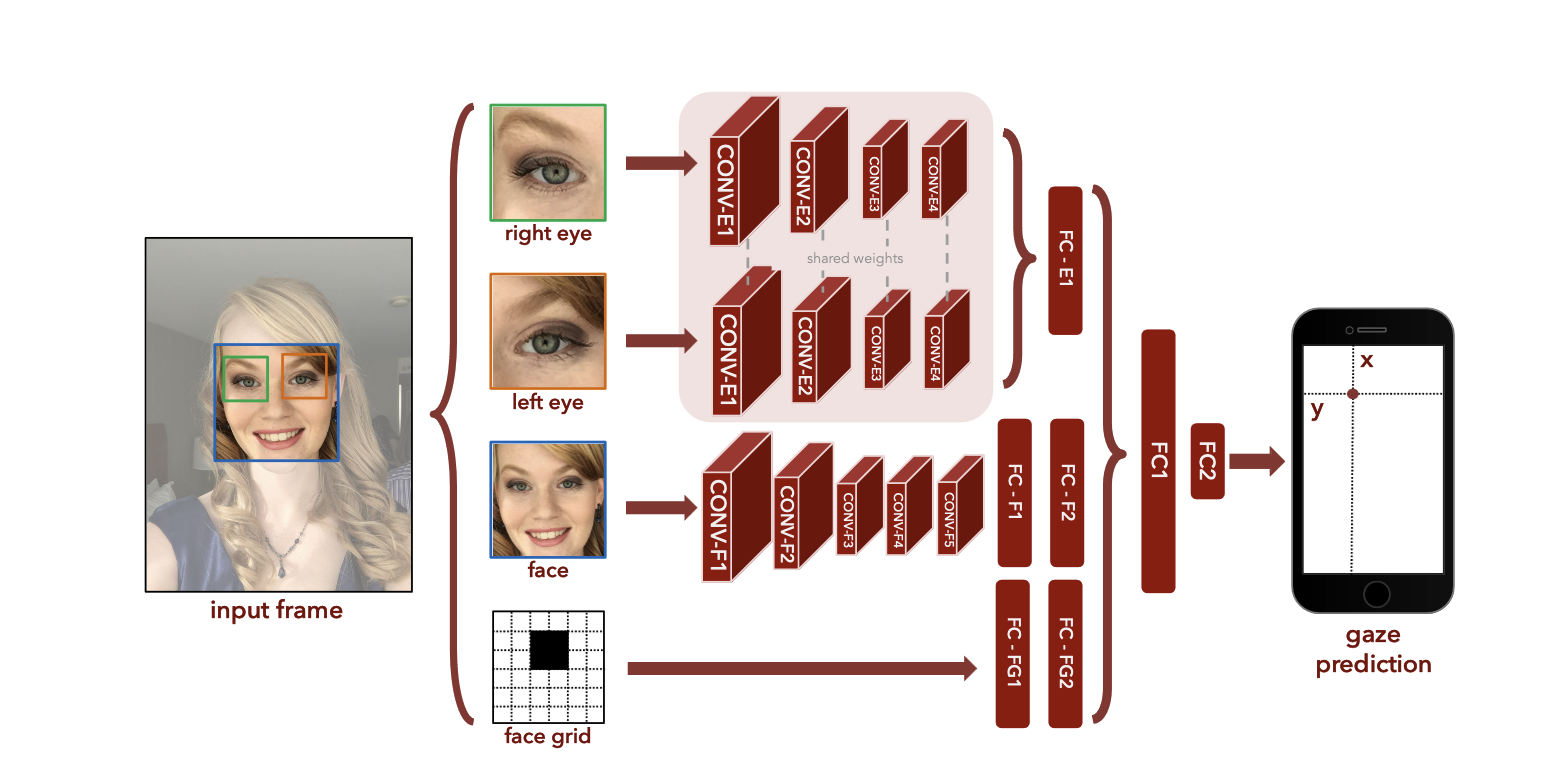
\includegraphics[scale=0.3]{../assets/iTracker-network.png}
    \end{center}
    \caption{The structure of the iTracker model, taken from ``Eye Tracking for Everyone'', 2016~\cite{krafka2016eye}}
    \label{fig:itracker-model}
\end{figure}

The only issue with using iTracker trained on the gazecapture dataset is that it was designed for gaze prediction on mobile devices. However, the repository~\cite{krafka2016eye,cheng2021survey} made available as part of their publication offered a configuration that allows the model to be trained on the MPII Face Gaze~\cite{zhang2019mpii} dataset, which captures the point of gaze information and images from people's laptops rather than phones as the gazecapture dataset does.

In the final release of my software, it will need to work on both mobile and desktop devices, and I have trained two models, one for clients on desktop devices and another for mobile devices.

In the literature, researchers highlight the importance of calibration for increased gaze mapping accuracy. Seonwook Part et al\.'s paper~\cite{seonwook2019fewshot} explains why this additional step is necessary for high-accuracy gaze mapping models, and introduces their FAZE (Few-shot Adaptive GaZE Estimation) framework which seeks to create a specialized model for a given user with a few shot approach. By training a generalized model on a few calibration points, their approach demonstrates significantly improved accuracy when compared to the generalized model. 

\section{Browser Extension Background}

Browser extensions allow users to modify the behaviour of their web browser. There are a number of reasons to install browser extensions, from improving the accessibility of webpages by changing their appearance and making use of ARIA tags~\cite{w3c2018accessible,lsdsoftware2024read}, to improving security through the use of password managers which enable users to generate and store secure passwords which are linked to a specific website and inserted into password fields automatically~\cite{lastpass}, and even ad blocker extensions which block advertisements on webpages~\cite{hill2014ublock}. These extensions run on top of webpages and allow developers to interact with almost every aspect of the page~\cite{frisbe2022building}, including network requests, the Document Object Model (DOM), and even access the digital currency wallets of users in some cases~\cite{finlay2015metamask}. 

The document object model represents an HTML document as a tree, which can be manipulated by scripts. This is a very powerful concept that has largely been responsible for the rise of dynamic web pages, also known as Web 2.0. Browser extensions make use of this to change the webpage as they see fit.  

In the early days of browser extensions, developers had to make use of proprietary APIs which were limited to a single browser. Thus, a distinct codebase was required for each browser they wanted the extension to be available on. In 2009, Google Chrome integrated its API for developing browser extensions with HTML, CSS, and Javascript. As Google Chrome rapidly became the most popular browser in 2012, other browsers implemented their API for their browser. This enabled developers to use a single codebase for an extension across multiple browsers. 

In every browser extension, there is a file known as the manifest. This file contains the metadata for the extension in the JavaScript Object Notation (JSON) format and includes keys such as author, background scripts, and a description of the extension behaviour~\cite{bengtsson2020manifest}. In 2020, the chromium developer team announced a new version of this file, known as manifest V3. This update provided many improvements to security, performance, and privacy~\cite{li2020manifest}. However, part of this update limited developers' access to network requests and ended the practice of remotely hosted code. While this does improve the security of browser extensions, it also limits the effectiveness of certain extensions which rely on being able to block certain network requests and remotely hosted code. Manifest V3 forces all extensions to contain all of their functionality within the extension itself, and not reach out to external services. 



\chapter{Methods}
\label{chap:methods}

% How the model was trained
% How the browser extension works
% How the extension communicates with the model
% How the model works
% Datasets

\section{Browser Extension}

I originally believed that developing an extension for Manifest V3 would significantly increase the complexity of development for my project. However, opting to use Manifest V2 would limit the potential user base of the system to Firefox users, which only make up approximately 3\% global browser traffic~\cite{statcounter2024browser}. I considered which would be the best approach to take, and eventually decided on developing my extension for the manifest V3 API, as it would allow virtually every web browser in the world to run the extension easily.

As part of my research, I discovered the Plasmo framework~\cite{plasmo}. This enables developers to rapidly develop cross-platform browser extensions. It handles all of the configuration and intricacies of developing browser extensions. I also found that when developing the extension, I was not hindered by any of the restrictions put in place by the Manifest V3 API.

The browser extension is activated on page load. Once the extension is loaded into the context of the webpage, it requests access to the user's webcam using the Media Capture and Streams API, which is a part of all major browsers and allows for the manipulation of audio and video streams. If the user does not allow access to the webcam, the extension will display a small notice on the page informing them that the extension will not function without these permissions. It then gets a list of all elements within the current viewport. The viewport is a concept which represents the visible area of a page. This list is then filtered based on the tag name, elements that contain text are kept, and others such as \texttt{<div>}, \texttt{<header>}, and \texttt{<section>} are discarded. This is necessary as a lot of HTML elements contain no text, 

The browser then waits until the page it's running on goes out of focus, meaning the user has switched browser tabs, and takes an image capture from the webcam. It passes that image, and some information about what kind of device the browser extension is running on, i.e.\ desktop or mobile device, to a local python server. The python server then performs inference on that image and passes the gaze location back to the browser extension, which then determines which element the gaze location intersects with, and highlights it. See Fig~\ref{fig:flowchart} for a graphical guide as to how the extension functions. 

\begin{figure}
    \begin{center}
        
\includegraphics[scale=0.25]{../assets/flowchart.png}
    \end{center}
    \caption{The flowchart outlining the functionality of the browser extension}
    \label{fig:flowchart}
\end{figure}

\section{Python Server}

I developed the Python server using FastAPI, a library built on top of Flask which allows rapid development of REST APIs. I chose to use FastAPI as I am already familiar with the framework due to the ease of use, and excellent performance~\cite{klenov2015benchmark}. Other, more performant frameworks exist for this use case such as BlackSheep~\cite{prevato2018blacksheep}, but I am unfamiliar with them, and they don't have as much community support behind them.  

The API only has two endpoints, one to verify that the server is running, and another to perform inference on an image. The image is encoded in the form data, meaning it is encrypted while in transit. It also takes a parameter telling the API which model to perform the inference on, the model trained on gazecapture for mobile devices, and the model trained on MPII face gaze for desktop devices. 

As the API runs locally on the user's device, there is no need for the content of the request to be encrypted. However, in a real-world deployment of this project, an SSL certificate should be obtained for the API to ensure malicious actors cannot intercept the images taken from the browser extension. 


\section{Model Selection}

When considering models, I wanted something that does not rely on any other systems, such as head pose detection, as adding additional inference would amplify errors between models and would make the predictions less accurate. For this reason, I opted to use an appearance-based model which predicts a 2D point of gaze. For this reason, I chose to use the iTracker model as outlined in~\cite{krafka2016eye}. This model has shown promising performance in both a desktop and mobile context, \(7.67\text{cm}\) for desktop applications, \(2.81\text{cm}\), \(1.86\text{cm}\) in tablet and phone environments respectively~\cite{cheng2021survey}.

\section{Datasets}

To develop the deep learning model, I used both the Gazecapture and MPIIFaceGaze datasets. 

\subsection{Gazecapture}

The Gazecapture dataset was collected through crowdsourcing. This allowed the authors to get a very high number of subjects ($1474$), and therefore a high number of images in the dataset ($2,445,504$). Participants were gathered using Amazon's Mechanical Turk service~\cite{mturk} and asked to download a free app on their device. The Mechanical Turk platform allows researchers and developers access to a large, diverse on-demand workforce. Once opened, the app asked the participants to enable airplane mode to avoid distractions while collecting the data. The app then displays a pulsating red dot on the screen for approximately 2 seconds~\cite{krafka2016eye}, and the camera begins recording 0.5 seconds after the dot is displayed, once the recording is complete, the dot disappears. The app then displays \textit{L} or \textit{R} on the screen for a short window of time, 0.05 seconds. The user must press either the left or right side of the screen depending on what label was displayed to measure their engagement with the application. If they get it wrong, they are warned and required to repeat the previous dot. The app also makes use of the real-time face detector built into iOS to ensure their face is visible in the video captures.

By making use of crowdsourcing to create datasets, the diversity of participants is significantly greater than researchers would otherwise get. Gazecapture has a wide variety of ethnicity, lighting conditions, head poses, appearance, and background among the participants, see Fig.~\ref{fig:gazecapture-sample}

\begin{figure}[h]
    \begin{center}
        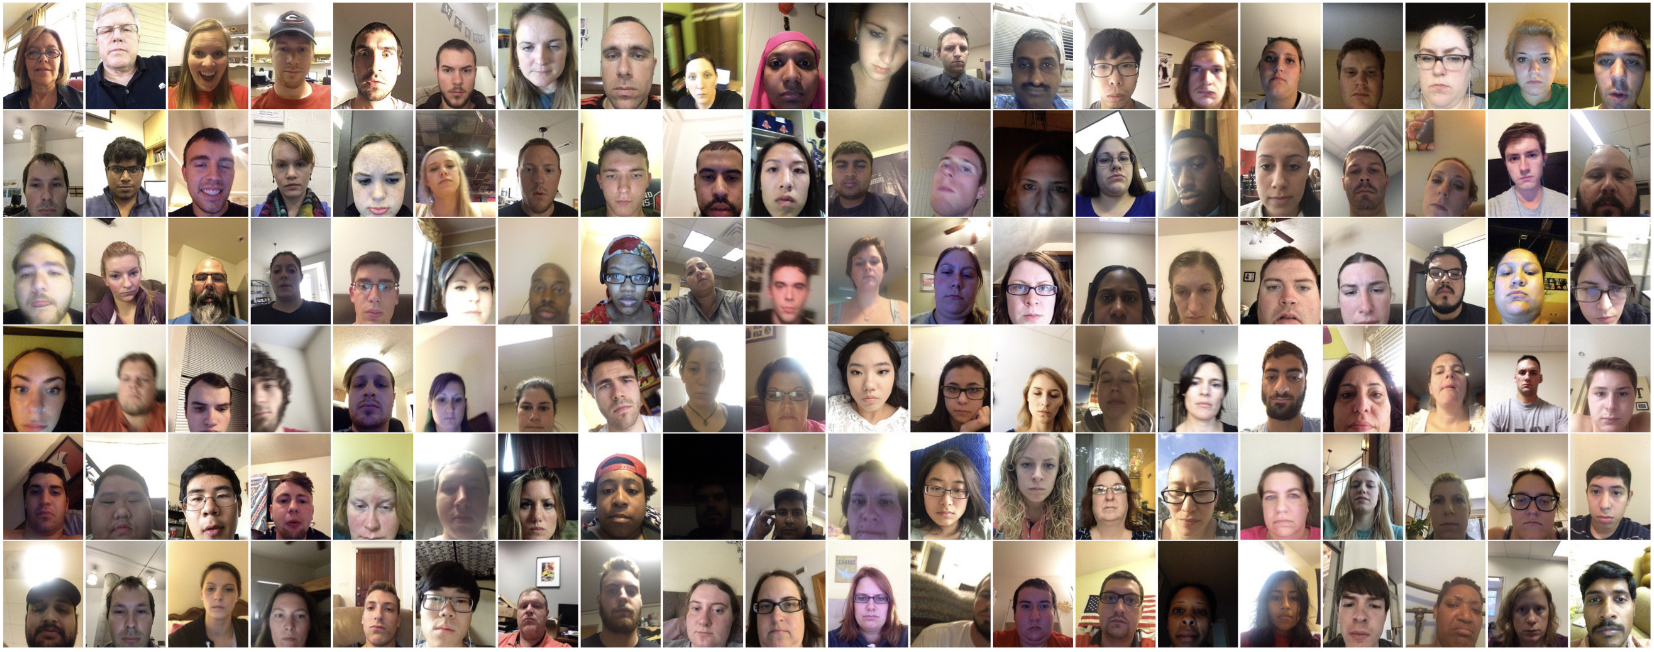
\includegraphics[scale=0.25]{../assets/Screenshot 2024-04-11 at 12.49.10.png}
    \end{center}
    \caption{Sample frames from the Gazecapture dataset, taken from~\cite{krafka2016eye}}
    \label{fig:gazecapture-sample}
\end{figure}

The dataset exhibits a wide variety in the head pose, and gaze directions when compared to other comparable datasets, such as TabletGaze~\cite{huang2016tabletgaze} and MPIIGaze~\cite{zhang15cvpr}, as exhibited in Fig.~\ref{fig:gazecapture-distribution}

\begin{figure}[h]
    \begin{center}
        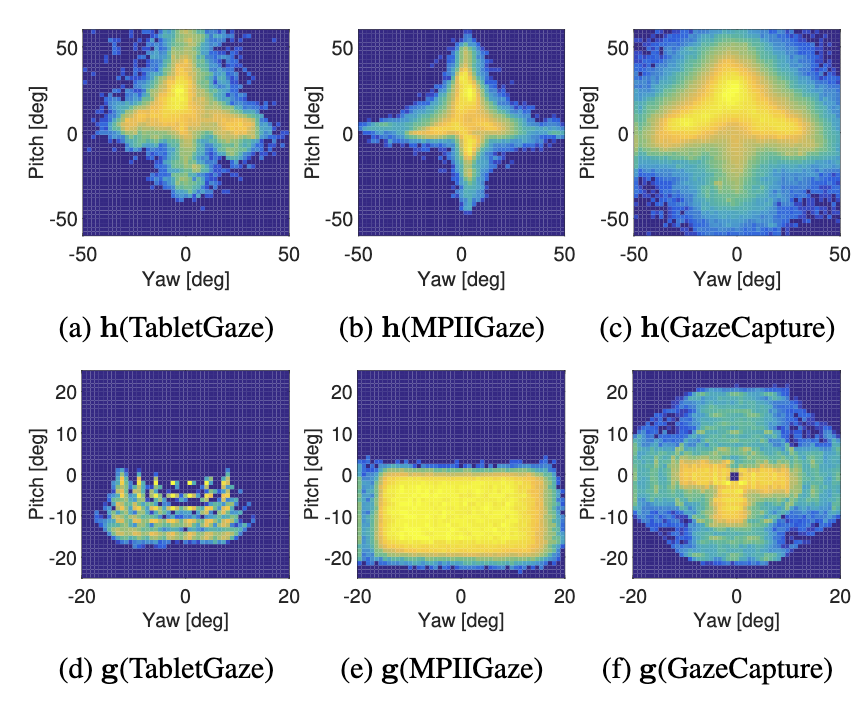
\includegraphics[scale=0.5]{../assets/Screenshot 2024-04-11 at 13.09.16.png}
    \end{center}
    \caption{Distribution of head pose \textbf{h} and gaze direction \textbf{g} relative to head pose for TabletGaze MPIIGaze, and Gazecapture. All intensities are logarithmic, taken from~\cite{krafka2016eye}}
    \label{fig:gazecapture-distribution}
\end{figure}

\subsection{MPIIFaceGaze}

I also trained a model on the MPII Face Gaze dataset~\cite{zhang2019mpii}. This dataset was captured from a smaller pool of participants (15) and considers gaze mapping within the context of devices such as laptops. The goals of this dataset were to capture images of participants outside of laboratory conditions and to record images of participants over a longer period. To achieve these goals, researchers opted to capture the data on participants' devices, as they typically are only operated by a single user throughout the day for a long period. As laptops can be used anywhere, the dataset exhibits wide variation in lighting conditions, and head pose from participants using their devices in a variety of environments. 

The dataset was collected using a background service running on their laptop. Every 10 minutes, the service would ask users to fixate on a random series of 20 on-screen positions. The ground truth data were collected using the moving dot stimulus as outlined in~\cite{kassner2014pupil}. The dots would slowly become more transparent. Once the dot was about to become fully transparent, the user was instructed to press the space bar to ensure their attention was focused on the dot. This method collected a total of 213659 images from 15 participants. 

The diversity of participants in comparison to gazecapture is significantly worse. Out of the 15 participants, only six were female, and a majority were White or Asian. Despite this, I chose to use this dataset as the iTracker model I use to perform inference. The repository~\cite{krafka2016eye,cheng2021survey} includes methods to process and load the data into the model. 

\subsubsection{Data Augmentation}

The MPIIFaceGaze dataset does not contain any subsets for testing and validation, so I had to create them myself. I decided on a 66.6/20/13.3\% split for training, validation, and testing. This split was performed on each participant to ensure the model didn't see any images of the participants within the training set. Members of each subset of the dataset were randomly selected. 

I also had to modify the ground truth data. I wanted the trained model to work on screens of any size, while the training data included a data point of the screen size in pixels divided by the screen size in millimeters, which was then divided by 100 and fed into the model, the web browser does not expose any behaviour to easily find the size of the screen in millimeters and thus made it difficult to get the true gaze location. I changed this ratio to the screen size in pixels, and then multiplied the gaze location, measured in pixels from the origin by the reciprocal of the screen size. This restricts the range of values the true gaze location can take to 0-1 and allows the model to learn the 2D gaze position for any screen size. 

After augmentation, some of the true gaze locations ended up lying outside of the screen. To remedy this, I clamped the ground truth data between 0 - 1 before feeding it into the model. This prevents the model from predicting gaze locations which lie outside of the screen, and in the worst case will end up opting for the bottom right of the screen. 

\section{Training}
\label{sec:training}

The training was performed on a single Mac Studio with an M1 Ultra Chip\footnote{I think it's an M1? Will check tomorrow} with 64GB of memory. Recent Apple systems offer a new set of tools known as Metal Performance Shaders (MPS) to rival Nvidia's CUDA platform, which allows developers to utilize the power of parallel processing and rapidly train neural networks. 

When training with MPIIFaceGaze, it took approximately 30 hours to perform 25 epochs, with a learning rate of 0.001. As we see in Fig.~\ref{fig:val}, the validation distance decreased practically every epoch, but not by very much. 

\begin{figure}
    \begin{center}
        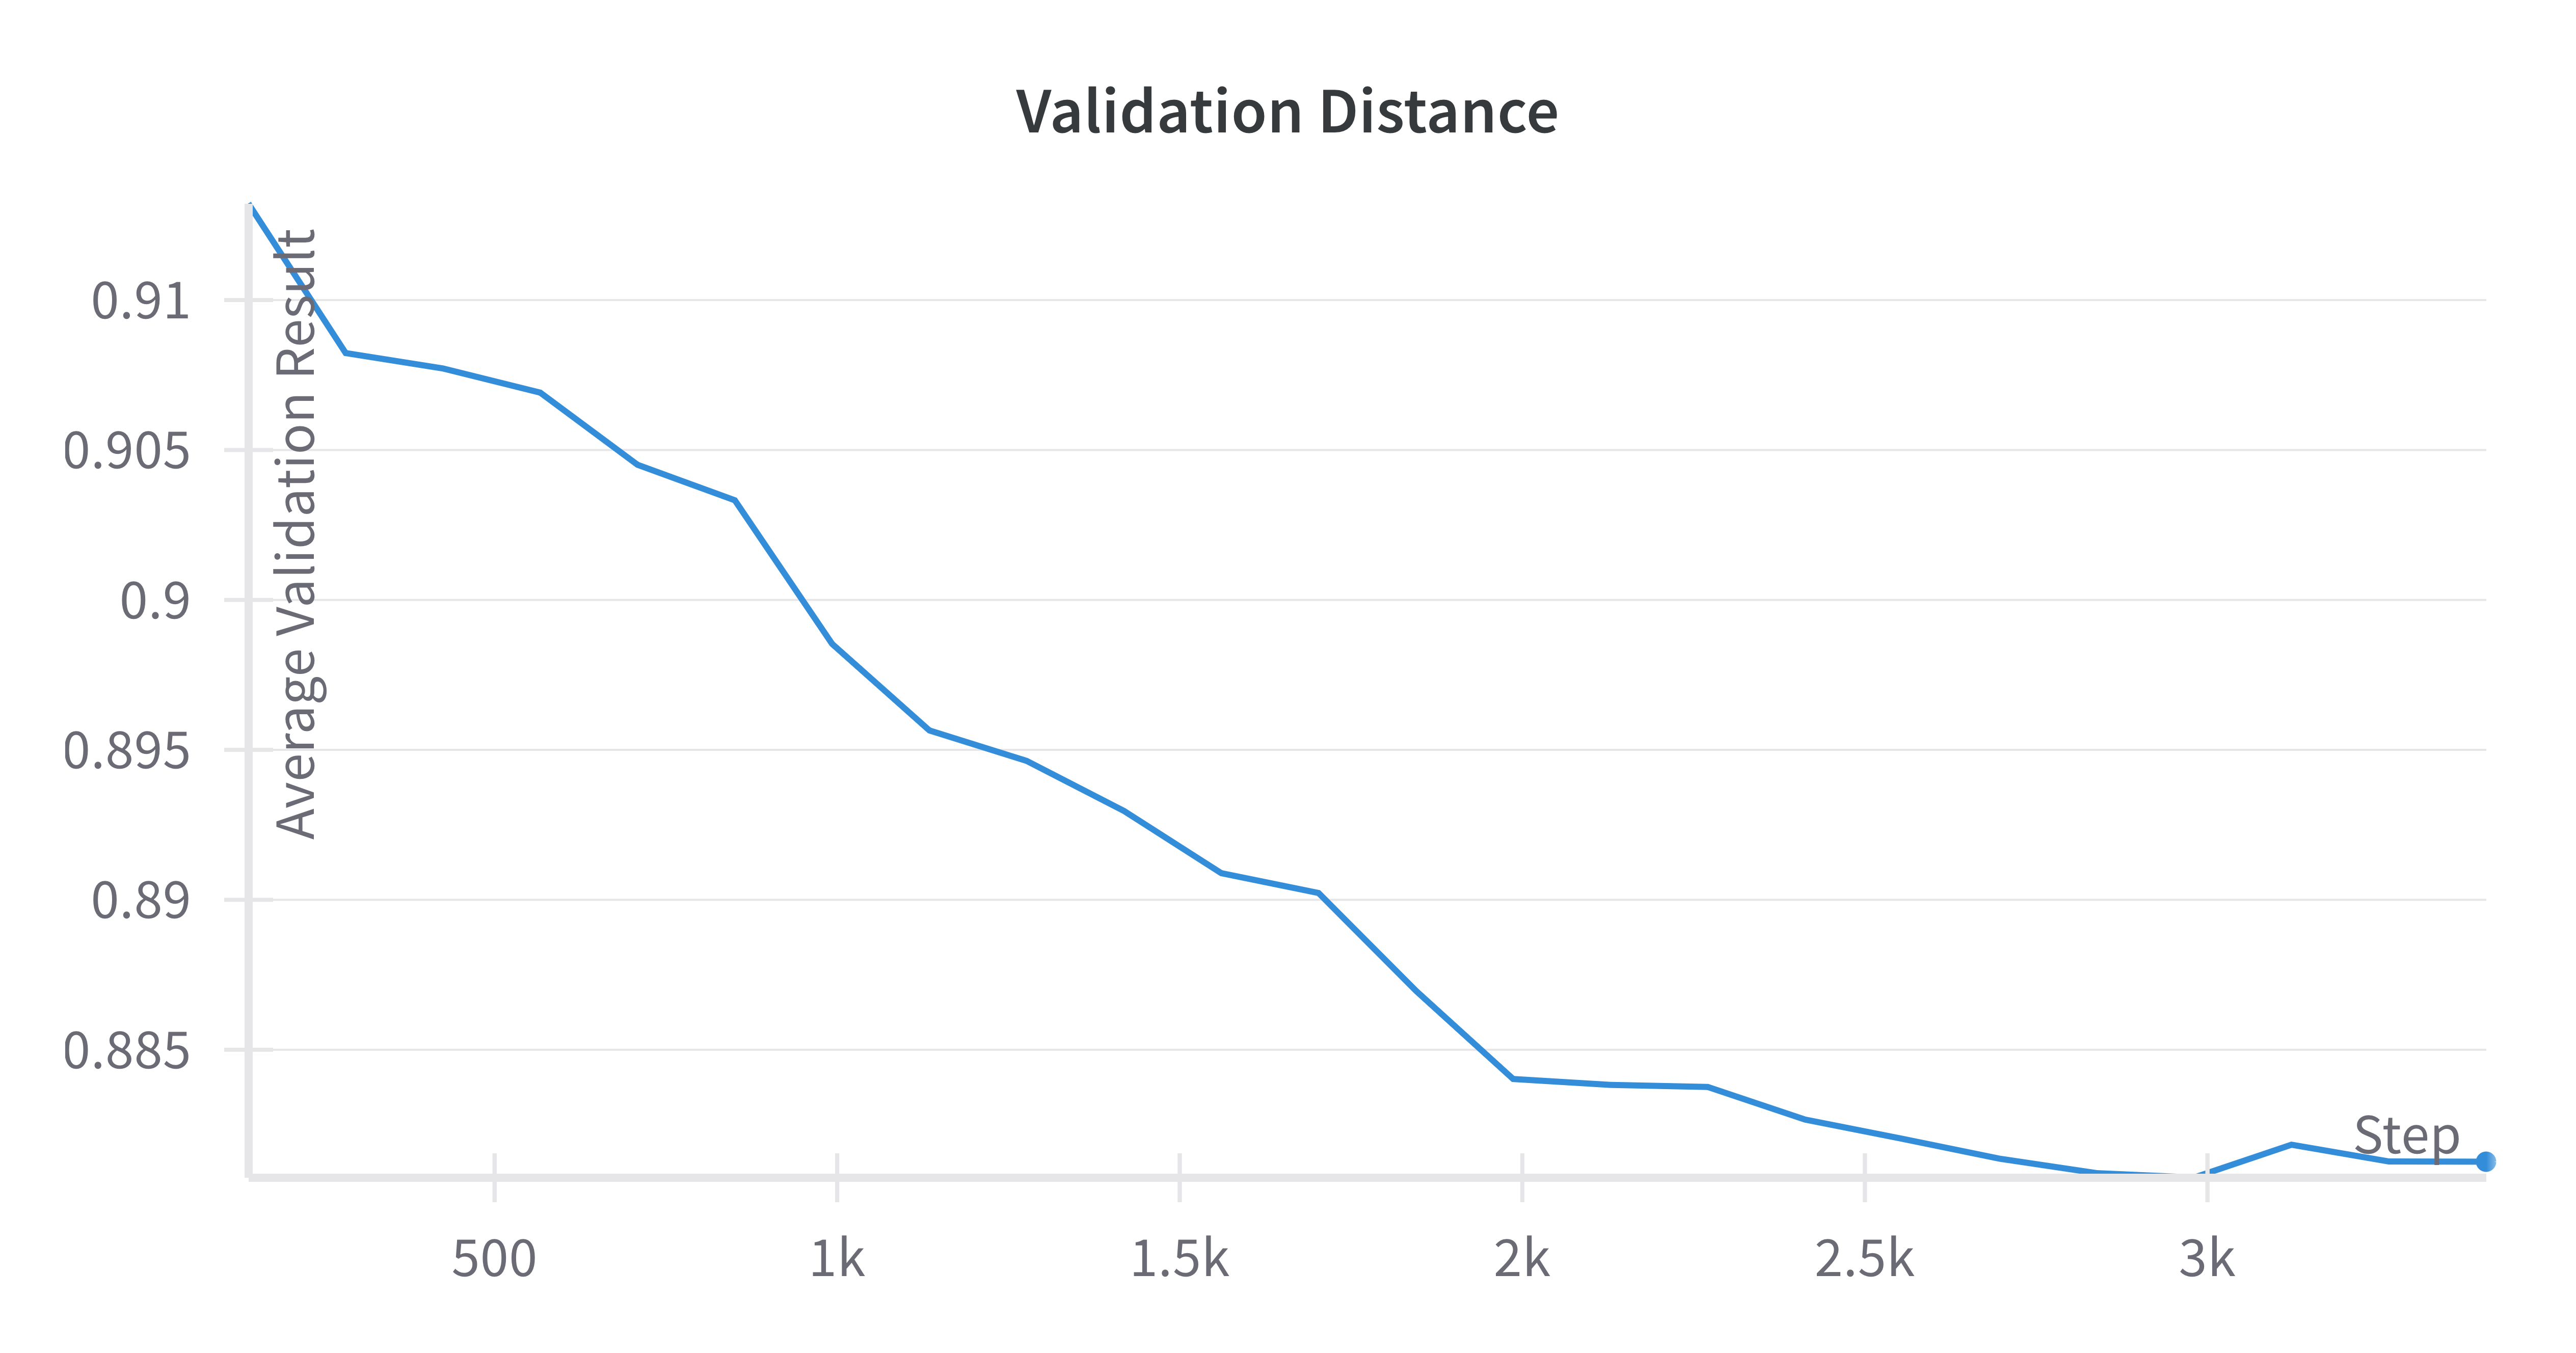
\includegraphics[scale=0.04]{../assets/mpii-val.png}
    \end{center}
    \caption{The average validation distance of iTracker with MPII Face Gaze}
    \label{fig:val}
\end{figure}

\subsection{Transfer Learning}

The two datasets I chose to use varied massively in terms of available data. MPIIFaceGaze has a total of 15 participants for a total of 45000 images, whereas Gazecapture has a total of 1474 participants with a total of 1490959 images. This made the training times for the two models drastically different, as discussed in Section~\ref{sec:training}, it took nearly 30 hours to perform 25 epochs of training on MPII Face Gaze. Using the same hardware, it would've taken nearly a month to perform a similar training run. 

For this reason, I chose to perform transfer learning on the model trained on MPII Face Gaze with a subset of the Gazecapture dataset. I chose to only modify the weights of the fully connected layer, and freeze all of the weights in the convolution layers. 

The use of transfer learning allows deep learning models to be adapted to a new domain, using a smaller dataset~\cite{koehrsen2018transfer}. 

\begin{itemize}
    \item MPII trained model avg dist. on MPII test \(0.8803248405456543\)
    \item MPII trained model avg dist on gazecapture test: \(7.583703517913818\)
\end{itemize}


\chapter{Results and Evaluation}

\begin{itemize}
    \item Comparing my models performance against other eye-tracking models
    \item How the overall project meets the requirements explored in Section. \ref{sec:specific-objectives}
    \item Whether the project meets the stretch objectives.
    \item
\end{itemize}

\chapter{Discussion}

\section{Datasets}

I initially planned on using 3 datasets, Gazecapture~\cite{krafka2016eye}, MPII Face Gaze~\cite{zhang2019mpii}, and ETH-X Gaze~\cite{zhang2020ethxgaze}. I initially wanted to merge each of these datasets into one large dataset which would increase the amount of data available to the model and hopefully increase its performance.

I believed merging the three datasets into one larger one would significantly increase the performance of my model as they all captured data in unique environments. Both Gazecapture and MPII Face Gaze were captured ``In-the-wild'', meaning data instances were collected in an uncontrolled environment, such as the participant's bedroom, a library or a coffee shop. This leads to the training data having a variety of lighting conditions but generally having limited variation in head pose~\cite{cheng2021survey}. This is most noticeable in the MPII Face Gaze dataset and is less of an issue in the Gazecapture dataset as subjects of this dataset were instructed to move their phone around as they completed the data collection. ETH-X Gaze however captures subjects in a controlled environment and captures 18 different angles concurrently. The authors also varied the lighting conditions when capturing data.

However, the ETH-X Gaze dataset did not include any annotations for 2D gaze targets. While I could've used the method outlined in~\cite{zhang15cvpr} to convert between a gaze direction vector and a pixel-wise gaze target, I was unable to find the time to implement this. Further work could add samples from this dataset into the training data to help the model better learn variations in both head pose and lighting conditions, despite the data being captured in a controlled setting. As the images were captured in a controlled setting, estimating the origin, and screen pose would be easier than converting 3D gaze vectors to gaze targets in an in-the-wild setting, as the origin and screen pose would be different in each instance. 

Training the model on this dataset would've also required the development of a custom data reader, which transforms the raw data into something that the model can understand. This requires the use of another machine learning model, such as the 68-point facial landmark shape predictor~\cite{king2015models} model offered by dlib~\cite{king2009dlib}, to crop certain elements of the face, such as the eyes, and face. 

\section{Gaze Estimation Model}

As explored in Section~\ref{chap:methods}, I made use of the iTracker model~\cite{krafka2016eye} to handle performing gaze location inference. This was because of its ability to learn gaze inference on images taken from a webcam or front-facing camera with very little pre-processing when compared to other models. However, further work could develop and evaluate the effectiveness of other, custom models based on state-of-the-art architectures found in the literature such as~\cite{seonwook2019fewshot,tafasca2023sharingan}. 

Further work could also research the effect of utilizing a 3D gaze vector model, such as~\cite{zaho2024gazeswin,yu2019deep} on the accuracy of the final product. I was unable to implement this myself as the process of converting between 3D gaze direction vectors requires estimating both the head pose of the user and the position of the screen within 3D space~\cite{zhang15cvpr}. However, further research could involve the prediction of these parameters. For example, making use of techniques such as Appearance template methods~\cite{niyogi1996example}, in which a new image of a head is compared to a set of examples labeled with a discrete pose to find the most similar pose, or detector array methods where a series of head detectors are trained on a specific pose and assign a discrete pose to the detector with the greatest support, among numerous other methods which are explored in~\cite{chutorian2009head}. Screen pose can be determined easily on mobile devices by making use of the gyroscopes that are present in nearly all modern smartphones. Desktop devices are less likely to have these sensors, as they are typically static while in use, which makes it far easier to estimate their pose in 3D space.

Another aspect of this project that should be explored is how well a pre-trained model performs. A variety of 


\begin{itemize}
    \item Would've been interesting to develop my own model
    \item Should've seen how the model performs with pre-trained models such as ResNet and others
\end{itemize}

\chapter{Conclusion}

\printbibliography

\end{document}